% 2D Distance from Point to Line Segment
%
% File:         2d-point-to-line-segment.tex
% Author:       Bob Walton (walton@acm.org)
% Date:      	Fri Dec 21 07:41:01 EST 2012
  
\documentclass{minimal}
\usepackage[paperheight=2.2in,paperwidth=2.4in,
            height=2.2in,hoffset=0.1in,
	    voffset=0.05in,left=0in,width=2.4in]{geometry}
\usepackage{color}
\usepackage[usenames]{xcolor}
\usepackage{scalefnt}
\usepackage[greek,english]{babel}
\usepackage{tikz}
\newcommand{\SMALL}{\scalefont{0.8}}
\newcommand{\THETA}{{\greektext J}}
\usetikzlibrary{arrows}
\begin{document}
\raggedright
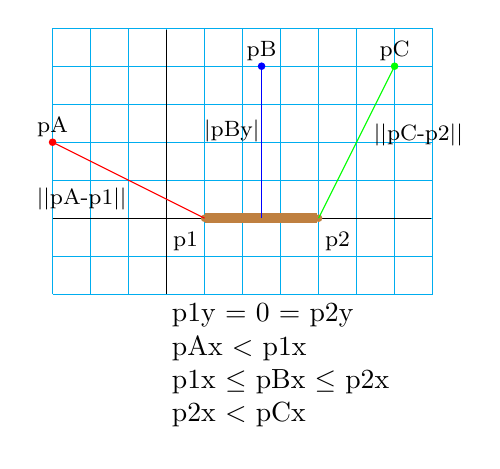
\begin{tikzpicture}[x=0.190in,y=0.190in]
\begin{scope}[yshift=1in,>=triangle 45,shorten >=0.01in]
    \draw[cyan] (-3,-2) grid[step=1] (7,5);
    \draw[black] (-3,0) -- (+7,0);
    \draw[black] (0,-2) -- (0,+5);

    \fill[brown] (1,0) circle(0.1) + (-0.5,-0.6) node[black]{\SMALL p1};
    \draw[brown,line width=0.05in] (1,0) -- (4,0);
    \fill[brown] (4,0) circle(0.1) + (+0.5,-0.6) node[black]{\SMALL p2};

    \fill[red] (-3,+2) circle(0.1) + (+0,+0.4) node[black]{\SMALL pA};
    \draw[red] (1,0) -- (-3,+2);
    \draw[black] (-1.0,0.5) + (+0.2,0) node[left]{\SMALL $||$pA-p1$||$};

    \fill[blue] (+2.5,+4) circle(0.1) + (+0,+0.4) node[black]{\SMALL pB};
    \draw[blue] (+2.5,0) -- (+2.5,+4);
    \draw[black] (2.5,2) + (+0.2,+0.3) node[left]{\SMALL $|$pBy$|$};

    \fill[green] (+6,+4) circle(0.1) + (+0,+0.4) node[black]{\SMALL pC};
    \draw[green] (4,0) -- (+6,+4);
    \draw[black] (5,2) + (+0.2,+0.2) node[right]{\SMALL $||$pC-p2$||$};
\end{scope}

\draw[black] (3,1.4) node {
    \begin{tabular}{l}
    p1y = 0 = p2y \\
    pAx $<$ p1x \\
    p1x $\le$ pBx $\le$ p2x \\
    p2x $<$ pCx \\
    \end{tabular}
};

\end{tikzpicture}
\end{document}



